\documentclass[conference]{IEEEtran}
\IEEEoverridecommandlockouts
% The preceding line is only needed to identify funding in the first footnote. If that is unneeded, please comment it out.
\usepackage{cite}
\usepackage{amsmath,amssymb,amsfonts}
\usepackage{algorithmic}
\usepackage{graphicx}
\usepackage{textcomp}
\usepackage{xcolor}
\usepackage[T1]{fontenc}
\usepackage[utf8]{inputenc} 
\usepackage{url} %Para conseguir colocar links
\usepackage{hyperref} %Para fazer um link clicável que leva até a figura/tabela correspondente.
\usepackage{booktabs} %Para usar as tabelas
\usepackage{amssymb}  % Para \checkmark
\usepackage{array}    % Para formatação de colunas
\usepackage{fancyhdr} % Para criar cabeçalhos e rodapés customizados
\usepackage{lastpage} % Para referenciar a última página do documento
\usepackage{balance} % Para balancear colunas
\usepackage[absolute,overlay]{textpos}
\usepackage{graphicx} % para rotatebox

\def\BibTeX{{\rm B\kern-.05em{\sc i\kern-.025em b}\kern-.08em
    T\kern-.1667em\lower.7ex\hbox{E}\kern-.125emX}}

\begin{document}

\title{A Forward Chaining Expert System for
Personalized Programming Language Selection
}

\author{\IEEEauthorblockN{Andi Sholihin}
\IEEEauthorblockA{\textit{Department of Informatics} \\
\textit{Institut Teknologi Sepuluh Nopember}\\
Surabaya, Indonesia \\
6025231080@student.its.ac.id}
\and
\IEEEauthorblockN{Shintami Chusnul Hidayati}
\IEEEauthorblockA{\textit{Department of Informatics} \\
\textit{Institut Teknologi Sepuluh Nopember}\\
Surabaya, Indonesia \\
shintami@its.ac.id}
}

\maketitle

% Cabeçalho da lateral
\begin{textblock*}{0cm}(0.1cm,3cm) % largura e posição na página
    \rotatebox{90}{\footnotesize
        2024 International Conference on Innovation and Intelligence for Informatics, Computing, and Technologies (3ICT) | 
        979-8-3315-3313-7/24/\$31.00 ©2024 IEEE | 
        DOI: 10.1109/3ICT64318.2024.1082463}
\end{textblock*}

% Cabeçalho e Rodapé
\thispagestyle{fancy} % Aplica o estilo fancy apenas na página atual.
% Útil se você quiser que a primeira página de um capítulo ou seção tenha um cabeçalho/rodapé diferente do restante.
\pagestyle{fancy} % Aplica o estilo fancy para todas as páginas seguintes do documento.
% Ele permite que você use cabeçalhos e rodapés personalizados usando o pacote fancyhdr.
\fancyhf{} % Limpa qualquer conteúdo pré-existente nos cabeçalhos (head) e rodapés (foot)
\fancyhead[CE,CO]{2024 International Conference on Innovation and Intelligence for Informatics, Computing, and Technologies (3ICT)} % Define o conteúdo do cabeçalho:
%CE → Center Even: centro das páginas pares
%CO → Center Odd: centro das páginas ímpares
\fancyfoot[CE,CO]{\large \thepage} % Define o conteúdo do rodapé:
%\thepage → insere o número da página atual.
\renewcommand{\headrulewidth}{0pt} % Remove a linha horizontal que normalmente aparece abaixo do cabeçalho (headrule).
%0pt significa que a linha não será desenhada.
\setcounter{page}{324} %Define o número da página atual para 324
\setlength{\footskip}{60pt} % diminui distância do número até a margem


\begin{abstract}
Choosing the right programming language is a critical decision for beginners in computer science because it greatly influences their learning experience and future opportunities. This paper presents an expert system designed to assist novices in selecting a programming language that aligns with their preferences and project requirements. The proposed system uses the forward chaining method, a robust approach to expert system development. It draws on comprehensive developer survey data from Stack Overflow, focusing on the top ten most popular programming languages. Our methodology involved formulating evaluative questions to create a decision-making framework supported by a rule-based table, which served as the foundation for the system’s knowledge base. Implemented in Python, the expert system achieved a relevance score of 90\%, demonstrating its effectiveness in simplifying the programming language selection process for beginners.
\end{abstract}

\begin{IEEEkeywords}
expert system, programming languages, forward chaining, interest determination
\end{IEEEkeywords}

\section{Introduction}
Selecting the appropriate programming language is a critical decision in software development because it significantly affects a project’s performance, maintainability, and scalability \cite{Spinellis2006}. The rapid evolution of technology has led to the proliferation of programming languages, each with its strengths, weaknesses, and ideal use cases \cite{Noone2018}. This diversity, coupled with the varying requirements of different projects, poses a considerable challenge, particularly for novices and students who need help identifying the most suitable language for their specific needs \cite{Kelleher2005}. The problem is further complicated by the dynamic nature of programming paradigms, industry standards, and trends that influence language popularity and applicability \cite{Perera2021}. \\
\indent An expert system, a computer program that captures the knowledge of human experts, offers a promising solution to this challenge \cite{Reddy2022}. Such systems are designed to replicate the decision-making abilities of human experts, providing recommendations and solutions to problems that typically require specialized knowledge \cite{Hidayati2021}. Expert systems can be invaluable in programming language selection, offering personalized guidance to users, especially beginners who may lack the experience to make independent decisions. \\
\indent The selection of an appropriate programming language has been extensively studied in the literature, and various decision support models have been proposed to guide users in making informed choices. Among the most prominent methodologies is the Analytical Hierarchy Process (AHP), widely applied to prioritize and evaluate criteria in programming language selection. Tavana \textit {et al}. \cite{Tavana2023} provided an in-depth analysis of AHP’s evolution, highlighting its flexibility in addressing complex decision-making problems across diverse fields, including software engineering. Similarly, Abdelnabi \cite{Abdelnabi2019} used AHP to create a decision model specifically for novice programmers focusing on data analytics applications, demonstrating its effectiveness in structuring and simplifying decision-making processes. However, while AHP and similar multi-criteria decision-making models, such as the one proposed by Maretto \textit {et al}. \cite{Maretto2022}, offer robust frameworks for decision-making, they often rely on static criteria that may not fully capture the dynamic nature of programming language trends and individual user needs. \\
\indent In recent years, there has been increasing interest in integrating machine learning and artificial intelligence into programming language selection models. Machine learning offers a distinct advantage by enabling the model to learn from large scale data, identifying patterns that may not be immediately evident through traditional approaches \cite{Hsieh2014}. Farshidi \textit {et al}. \cite{Farshidi2021} introduced a decision model incorporating a detailed analysis of programming language ecosystems across various industry case studies to provide insights into how language selection impacts software quality and project success. Similarly, Ezenwoye \cite{Ezenwoye2018} explored the challenges of selecting an introductory programming language in educational contexts, emphasizing the need for adaptable systems that cater to diverse learning environments. These studies underscore the importance of flexibility and adaptability in decision support systems, which aligns with the motivation underlying our proposed expert system. \\
\indent In addition, Jain \textit {et al}. \cite{Jain2020} examined the environmental impact of programming language selection and introduced a novel perspective on how language choice affects CO2 emissions—a consideration that may become increasingly relevant as sustainability becomes a key concern in software development. The importance of context-specific factors was further highlighted by Katzy \textit {et al}. \cite{Katzy2023} and Li \textit {et al}. \cite{Li2021}, who investigated the implications of language selection in machine learning models and multi-language software projects, respectively. These studies suggested that a one-size-fits-all approach is insufficient for programming language selection, thus reinforcing the need for personalized, context-aware recommendations. \\
\indent Our proposed expert system distinguishes itself from existing approaches by leveraging forward chaining to provide personalized, dynamic recommendations. Unlike AHP-based models, which depend on predefined criteria, the proposed system can adapt to the user’s evolving needs and the changing landscape of programming languages. The forward chaining method, as discussed by \.{I}mamo\u{g}lu and Çetinkaya in the context of rule-based decision support systems \cite{Imamoglu2017}, allows for a more interactive and iterative decision making process in which the system gathers information progressively and refines its recommendations based on user input. \\
\indent Furthermore, the proposed system is designed to be accessible to beginners, addressing the challenges highlighted by Ahmed \textit {et al}. \cite{Ahmed2021} and Shrestha \textit {et al}. \cite{Shrestha2020} regarding the readability, writability, and reliability of programming languages and the difficulties developers face when learning new languages. By focusing on user-specific preferences and project requirements, our system simplifies the decision making process and enhances the learning experience, providing a tailored pathway for novices to navigate the diverse landscape of programming languages. \\
\indent In summary, while existing studies have laid a strong foundation for programming language selection through various decision support models and contextual analyses, our proposed expert system offers a novel approach that combines the adaptability of forward chaining with a user-centric design. This enables more personalized and context-sensitive recommendations, making it a valuable tool for beginners and experienced developers in rapidly evolving software development. \\
\indent The remainder of this paper is organized as follows. Section II describes the methodology employed in developing the expert system, including the formulation of evaluative questions, construction of the knowledge base, and implementation of the forward chaining inference mechanism. Section III presents the experimental setup and results, including an analysis of user feedback collected from a survey. Finally, Section IV concludes the paper by summarizing the key contributions of this study.
\section{Methodology}
\indent This section outlines the proposed systematic approach, identifying the most popular programming languages through developer surveys and formulating selection rules for programming languages.

\subsection{Identification of Popular Programming Languages}
\indent To enhance the credibility and relevance of this study, we used an annual developer survey conducted by Stack Overflow\footnote{\url{https://survey.stackoverflow.co/2023}}, an online platform for programmers worldwide. This survey was the primary source to determine the popular 
\begin{figure}
  \centering %Centraliza a figura dentro da coluna.
  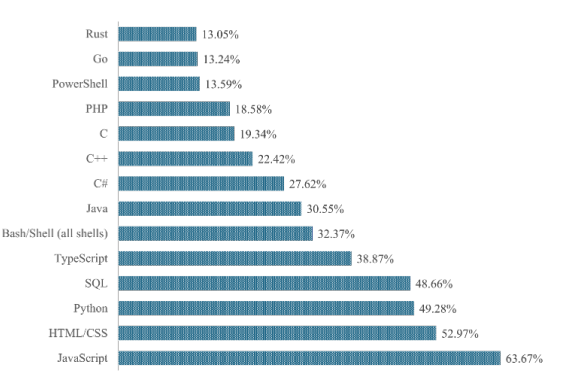
\includegraphics[width=\linewidth]{images/language_graphic.png} % [width=\linewidth] ajusta a largura da imagem à largura da coluna (ótimo para artigos em duas colunas).
  \caption{The identified most popular programming languages.} %Legenda
  \label{fig:languages} % Cria uma etiqueta para você poder referenciar depois com \ref{fig:languages}.
\end{figure}

\noindent programming languages in the current industry landscape, as summarized in Fig.~\ref{fig:languages}. Through a detailed analysis of the survey data, we identified prevailing trends and preferences among developers regarding their choice of programming languages. The insights gained from this analysis form a foundation for the subsequent development of programming language selection rules, thus bridging empirical data with practical application in our expert system.
\subsection{Formulation of Programming Language Selection Rules}
\indent Establishing robust criteria for selecting programming languages is critical in developing our expert system, which leverages the forward chaining method. The foundational step in this process involved creating evaluative questions designed to capture user requirements and preferences in programming language selection. These questions were crafted to align with key decision-making factors, ensuring their relevance and applicability. \\
\indent Based on analyzing Stack Overflow survey data, we identified the top ten programming languages that reflect current industry trends. These languages include JavaScript, Python, TypeScript, Java, C\#, C++, C, PHP, Go, and Rust. Table~\ref{tab:tabela}
presents a set of questions outlining the suitability of these languages for various software development tasks and programming paradigms.
\subsection{Implementation of Forward Chaining}
Creating a forward chaining inference system based on the provided table begins by defining a knowledge base comprising initial facts and a set of rules. The facts represent user responses to the evaluative questions, such as whether users wanted to develop a web frontend or work on data science projects. Each rule in the knowledge base corresponds to a row in the table and is structured as an “if-then” statement: if a user’s response satisfies a condition (e.g., “Yes” to developing a web frontend), then the programming languages deemed suitable for that task (e.g., JavaScript, TypeScript) are identified. Fig.~\ref{fig:flowchart} outlines the steps involved in the inference

\begin{table*}[h!] % O asterisco (float) indica que é uma tabela de largura total da página, mesmo em documentos de duas colunas
\centering % Centraliza a tabela horizontalmente na página
\caption{Programming Language Selection Rules} % Adiciona legenda/título à tabela  % Será automaticamente numerada
\label{tab:tabela}
\begin{tabular}{cp{5.3cm}ccccccccccc} % Define a estrutura das colunas
% c - Primeira coluna: centralizada (para o ID "Q01", "Q02", etc.)
% p{5.5cm} - Segunda coluna: parágrafo fixo de 5.5cm de largura (para as perguntas longas)
% cccccccccc - 11 colunas centralizadas
\toprule
ID & Question & JavaScript & Python & TypeScript & Java & C\# & C++ & C & PHP & Go & Rust \\
\midrule
Q01 & Do you want to develop a web frontend? & \checkmark & $\times$ & \checkmark & $\times$ & $\times$ & $\times$ & $\times$ & $\times$ & $\times$ & $\times$ \\
Q02 & Do you want to develop a web backend? & \checkmark & \checkmark & \checkmark & \checkmark & \checkmark & \checkmark & \checkmark & \checkmark & \checkmark & \checkmark \\
Q03 & Do you want to develop Desktop Applications? & \checkmark & \checkmark & $\times$ & \checkmark & \checkmark & \checkmark & \checkmark & $\times$ & \checkmark & $\times$ \\
Q04 & Do you want to develop Mobile Applications? & \checkmark & \checkmark & \checkmark & \checkmark & \checkmark & \checkmark & $\times$ & $\times$ & \checkmark & $\times$ \\
Q05 & Do you want to develop Games? & \checkmark & \checkmark & \checkmark & \checkmark & \checkmark & \checkmark & $\times$ & $\times$ & \checkmark & $\times$ \\
Q06 & Do you want to develop AI? & \checkmark & \checkmark & $\times$ & \checkmark & \checkmark & \checkmark & $\times$ & $\times$ & \checkmark & $\times$ \\
Q07 & Do you want to develop Data Science? & \checkmark & \checkmark & $\times$ & \checkmark & \checkmark & \checkmark & $\times$ & $\times$ & \checkmark & $\times$ \\
Q08 & Do you want to develop Big Data? & \checkmark & \checkmark & $\times$ & \checkmark & \checkmark & \checkmark & $\times$ & $\times$ & \checkmark & $\times$ \\
Q09 & Do you want to use an application that supports Object Oriented Programming? & \checkmark & \checkmark & \checkmark & \checkmark & \checkmark & \checkmark & $\times$ & \checkmark & \checkmark & \checkmark \\
Q10 & Do you want to use an interpreter-based programming language? & \checkmark & \checkmark & $\times$ & $\times$ & $\times$ & $\times$ & $\times$ & \checkmark & $\times$ & $\times$ \\
Q11 & Do you want to use a Compiler based programming language? & $\times$ & $\times$ & \checkmark & \checkmark & \checkmark & \checkmark & $\times$ & $\times$ & \checkmark & \checkmark \\
\bottomrule
\end{tabular}
\end{table*}
\begin{figure}[h!]
    \centering
    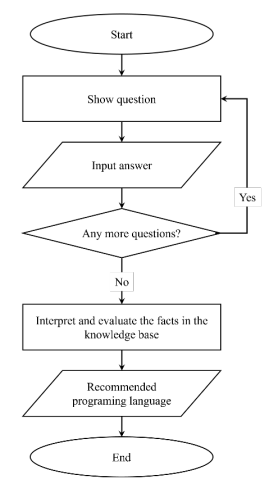
\includegraphics[width=0.27\textwidth]{images/flowchart.png}
    \caption{Flowchart of the inference procedure.}
    \label{fig:flowchart}
\end{figure}
procedure and Fig.~\ref{fig:questions} provides a sample inference using an ”if-then” rule.
\\
\indent The inference engine begins by collecting user input through a series of questions, each designed to capture user requirements and preferences for programming languages. As the user answers each question, these responses are stored as facts in the system. The forward chaining process begins by iteratively evaluating each rule in the knowledge base against the accumulated facts. When a match is found\textemdash meaning the user’s facts satisfy a particular rule\textemdash the rule is activated, and the corresponding programming languages are added to the list of recommendations.
\\
\indent As the system processes all relevant rules, it compiles a comprehensive list of programming languages that align 
\begin{figure}[t!]
    \centering
    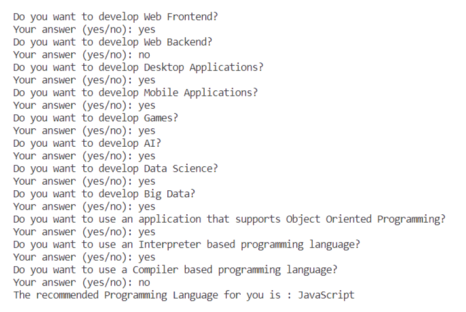
\includegraphics[width=0.45\textwidth]{images/questions.png}
    \caption{A sample of the inference using an“if-then” rule.}
    \label{fig:questions}
\end{figure}
with user requirements. If multiple languages are suitable, the system may present all options or prioritize them based on additional criteria, such as popularity or ease of learning. The final recommendations are then presented to the user, who can select the language that best suits their project goals. This process not only aids in making informed decisions but also provides an interactive experience where users can refine their choices according to their evolving preferences.
\section{Results And Discussion}
\indent We conducted a series of experiments involving student participation to assess the effectiveness of the developed expert system for programming language selection. The initial step involved inviting students to interact with the proposed system, which allowed them to answer several questions and receive recommendations for programming languages that best suited their needs. After using the system, we gathered feedback from 20 students through a survey designed to evaluate the relevance
of the recommendations provided by the system.
\\
\indent The survey results, which are shown in Fig.~\ref{fig:graphic}, offer insights into the system’s performance based on direct user feedback. The majority of respondents responded positively to the system’s usefulness, with 14 out of 20 students (70\%) finding
\begin{figure}[t!]
    \centering
    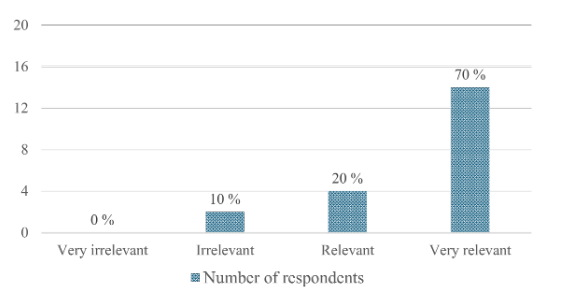
\includegraphics[width=0.4\textwidth]{images/graphic.png}
    \caption{Relevance scores obtained from the survey.}
    \label{fig:graphic}
\end{figure}
the proposed system “very relevant” in helping them choose a programming language that matched their needs. Additionally, four students (20\%) considered the system “relevant”, while only two students (10\%) felt that the system was “not relevant” for programming language selection. Notably, none of the respondents rated the system as “very irrelevant”.
\\
\indent The overwhelming positive response suggests that the expert system is generally well received and is considered a valuable tool to support decision-making in programming language selection. The lack of any ratings for “very irrelevant” further underscores the system’s perceived effectiveness among participants. Therefore, it is understand that the proposed system can be effectively utilized as a supportive resource to help users make informed choices about programming languages. 
\\
\indent To quantify the relevance of the system based on user ratings (very relevant = 4, relevant = 3, not relevant = 2, very irrelevant = 1), we calculated the overall percentage of the relevance score $\mathfrak{R}$ using the following formula:
\[
\mathfrak{R} = \frac{\sum_{i=1}^{n_r} s_i}{n_r \times \max_i(s_i)} \times 100\%,
\]
where $n_r$ is the number of respondents and $s_i$ is the relevance score given by participant $i$. Given that the maximum relevance value max$_i$ ($s_i$) is 4 (very relevant) and from the survey that 14 respondents indicated ”very relevant,” 4 indicated ”relevant,” 2 indicated ”not relevant,” and none indicated ”very irrelevant”, our relevance score $\mathfrak{R}$ is 90\%.
\\
\indent Therefore, the survey results demonstrate that the programming language selection expert system is highly relevant. This high percentage indicates strong user confidence in the system’s effectiveness in assisting with the programming language selection.
\\
\indent Despite the promising results, the current proposed system has some limitations that should be addressed in future research. Firstly, the system’s effectiveness was evaluated using a relatively small sample size of 20 students, which may limit the generalizability of the findings. Future studies should involve a larger and more diverse group of participants, including professionals and educators, to obtain a more comprehensive evaluation of the system’s relevance and utility across different user demographics. Secondly, the system relies on a predefined set of questions and rules, which may not capture the full range of programming language preferences and requirements across various domains. Incorporating machine learning techniques could allow the system to adapt and improve over time based on user feedback and evolving trends in programming language usage. Finally, the system currently evaluates programming languages based on general criteria, without accounting for specific project types or industry standards. Future research could explore the integration of domain-specific factors \cite{Thang2016}, \cite{Takayanagi2024}, such as industry-specific language requirements, performance benchmarks, and long-term maintainability considerations, to provide more nuanced recommendations.

\section{Conclusion}
This study introduced an expert system for programming language selection, employing forward chaining to provide personalized recommendations. Aimed at addressing the challenges faced by beginners in choosing the most suitable programming language, the system integrates a dynamic knowledge base that adapts to evolving industry trends and user needs. Our evaluation revealed that the system is highly effective, achieving a 90\% relevance score. The majority of users found the system valuable in assisting their programming language decisions, underscoring its potential as a practical tool for both novice and experienced developers.

\section*{Acknowledgment}

This work was partially supported by Institut Teknologi Sepuluh Nopember under Grant No. 1409/PKS/ITS/2023.

%Referências
\balance %para balancear as colunas
\bibliographystyle{IEEEtran}
\bibliography{references}

\end{document}
